\documentclass{wx672article} % $HOME/texmf/tex/latex/wx672article.cls

\usepackage{wx672cjk}
\usepackage[NoDate]{currvita}

\newlength{\outerbordwidth}
\pagestyle{empty}
\raggedbottom
\raggedright
%\usepackage[svgnames]{xcolor}
\usepackage{framed}
\usepackage{tocloft}



%-----------------------------------------------------------
%Edit these values as you see fit

\setlength{\outerbordwidth}{3pt}  % Width of border outside of title bars
\definecolor{shadecolor}{gray}{0.75}  % Outer background color of title bars (0 = black, 1 = white)
\definecolor{shadecolorB}{gray}{0.93}  % Inner background color of title bars


%-----------------------------------------------------------
%Margin setup

\setlength{\evensidemargin}{-0.25in}
\setlength{\headheight}{0in}
\setlength{\headsep}{0in}
\setlength{\oddsidemargin}{-0.25in}
\setlength{\paperheight}{11in}
\setlength{\paperwidth}{8.5in}
\setlength{\tabcolsep}{0in}
\setlength{\textheight}{9.5in}
\setlength{\textwidth}{7in}
\setlength{\topmargin}{-0.3in}
\setlength{\topskip}{0in}
\setlength{\voffset}{0.1in}


%-----------------------------------------------------------
%Custom commands
\newcommand{\resitem}[1]{\item #1 \vspace{-2pt}}
\newcommand{\resheading}[1]{\vspace{8pt}
  \parbox{\textwidth}{\setlength{\FrameSep}{\outerbordwidth}
    \begin{shaded}
\setlength{\fboxsep}{0pt}\framebox[\textwidth][l]{\setlength{\fboxsep}{4pt}\fcolorbox{shadecolorB}{shadecolorB}{\textbf{\sffamily{\mbox{~}\makebox[6.762in][l]{\large #1} \vphantom{p\^{E}}}}}}
    \end{shaded}
  }\vspace{-5pt}
}
\newcommand{\ressubheading}[4]{
\begin{tabular*}{6.5in}{l@{\cftdotfill{\cftsecdotsep}\extracolsep{\fill}}r}
		\textbf{#1} & #2 \\
		\textit{#3} & \textit{#4} \\
\end{tabular*}\vspace{-6pt}}
%-----------------------------------------------------------


\begin{document}
\begin{cv}{蒲启元}
  \vspace*{-1ex}
  {\small 能编写一个简单的操作系统}\\[2ex]
  \begin{tabular}{r@{\,:\,}l}%
    {\scriptsize\fa }&\emph{pqy7172@gmail.com} \\%
    {\fa }&\emph{18314555392}\\%
    
  \end{tabular}


  
  \vspace*{\dimexpr-1.5in-\topmargin-\headsep-\headheight-\baselineskip}%
  \hspace*{\dimexpr-1in-\evensidemargin-\parindent}%
  \hspace*{-10ex}
  \makebox[\paperwidth][r]{\frame{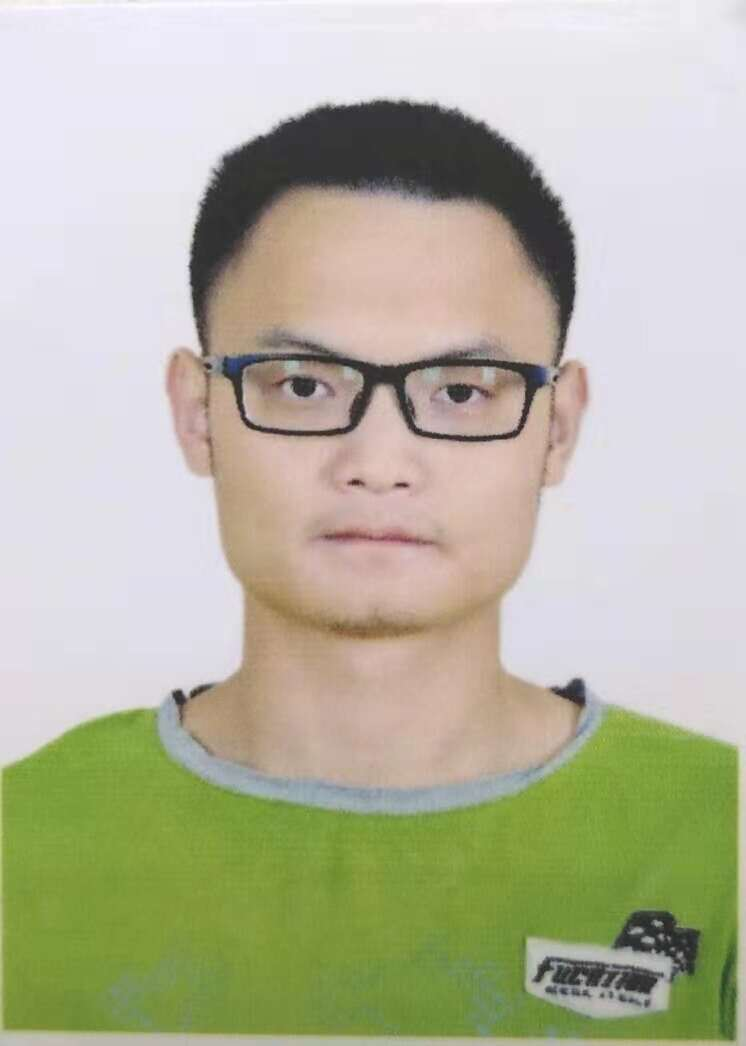
\includegraphics[width=0.15\textwidth]{me3}}}

  

    
    \begin{cvlist}{教育背景}
  \item[09/2014 -- 06/2018] 西南林业大学,大数据与智能工程学院,计算机科学与技术专业,本科
    生
    \begin{itemize}
    \item 主修课程:数据结构,操作系统,组成原理,网络等。这几门主要课程均是90分以上。
    \item 其中大三上学期作为学校交换生前往泰国学习。
    \end{itemize}
  \end{cvlist}

  \begin{cvlist}{开发经验}
  \item[RongOS --- 一个简单操作系统的实现]\ \par
    本项目从零开始编写了一个简单的操作系统。实现的功能包括多任务、内存管理、进程管理、窗口
    管理等。本项目也是我的毕业设计,并获优秀毕业论文奖。
    \begin{itemize}
    \item \url{https://github.com/Puqiyuan/RongOS}
    \item \url{https://github.com/Puqiyuan/RongOS/blob/master/doc/thesis/thesis.pdf}
    \end{itemize}
  \item[清橙网编程挑战] \ \par
    这个项目是独立自主完成清橙编程题目以训练编程能力。目前所完成的题目都是满分通过。另有其
    它类似的题解练习,包括两个C程序,高精度(小数点前后各可达999位)浮点计算器,操作系统中
    银行家算法等,基本上代表了目前我的最高编程能力。
    \begin{itemize}
    \item \url{https://github.com/Puqiyuan/Tsinsen_ACM}
    \item \url{https://github.com/Puqiyuan/URI_ACM}
    \item
      \url{https://github.com/Puqiyuan/High_Accuracy_Float_Calculator/blob/master/Calculator.c}
    \item
      \url{https://github.com/Puqiyuan/OS_Algorithms/blob/master/BankerAlgorithm/Programs/banker.c}
    \end{itemize}
  \item[UNIX环境高级编程] \ \par
    包括文件、目录、标准I/O、系统数据文件和信息、进程环境、进程控制、进程关系、信号、
    线程、线程控制、守护进程、进程通信、网络IPC等。Linux下的C开发是我想要从事的方向,未来的
    职业期望也就是Linux系统/后台开发。
    \begin{itemize}
    \item \url{https://github.com/Puqiyuan/APUE}
    \end{itemize}
  \end{cvlist}
  \begin{cvlist}{自我评价}
  \item[] 通过大学四年养成了一系列优秀的学习、工作、生活习惯,包括:
    \begin{enumerate}
    \item 熟练使用Google英文搜索解决各种问题,英文就是我的工作语言。
    \item 高效的命令行工作方式。
    \item 熟练使用Linux下的成套工具,包括Emacs,Vim,Latex,Org-Mode,Makefile,Github等。
    \item 熟练的C编程,具有三年Debian Linux使用配置经验,有一定的Bash Shell编程经验,
      对Linux下的C开发有一定的了解。
    \item 行事(编程)条分缕析,条理清楚,逻辑感强,细致追求完美。
    \item 坚持每周十或二十公里长跑。耐心与毅力之于技术问题的解决具有决定作用。
    \end{enumerate}
    总结起来,大学期间,虽然没有多少实际商业项目经验,但是看的专业书较多,自己独立写的代码
    不少,最大的特点是爱钻研好学,在刚开始工作时,虽无多少经验,但拥有这些基础能力,好的学
    习习惯,才有足够的后劲来持续学习发展,我相信这些习惯和学习能力会使我行稳致远。
  \end{cvlist}
  \begin{cvlist}{个人荣誉}
  \item[2014 — 2015] 年度校级三好学生
  \item[2015 — 2016] 年度省级三好学生
  \item[2018] 优秀毕业生,优秀毕业论文(设计)
  \item[] 云南省大学生计算机作品赛二等奖
  \end{cvlist}
\end{cv}
\end{document}








%%% Local Variables:
%%% mode: latex
%%% TeX-master: t
%%% End:
